\section{Hadoop y Spark}

\subsection{Hadoop}

\textit{Apache Hadoop software library} es un \textit{framework} que permite el procesamiento de grandes volúmenes de datos a través de \textit{clusters} de computadoras usando un modelo de programación simple.Esta diseñado para escalar de servidores individuales a miles de maquinas, cada una ofreciendo procesamiento local y almacenamiento.

\subsubsection{Arquitectura de Hadoop} 
	El núcleo de Apache Hadoop posee dos módulos principales:
	
	\paragraph{YARN} \textit{Yet Another Resource Negotiator (YARN)} asigna CPU, memoria y almacenamiento a las aplicaciones que se ejecutan en un cluster Hadoop. La primera generación de Hadoop sólo podía ejecutar aplicaciones MapReduce. YARN permite que otros marcos de aplicaciones (como Spark) también puedan ejecutarse en Hadoop.\cite{yarn}

	El planteamiento fundamental de YARN es dividir las funcionalidades asociadas al manejo de recursos y el monitoreo/planeación de trabajos (\textit{jobs}) en demonios separados. La idea es tener de forma global un \textit{ResourceManager} (RM) y por cada aplicación un \textit{ApplicationMaster} (AM). Una aplicación representa uno o muchos trabajos.\cite{horyarn} 
	El \textit{ResourceManager} y el \textit{NodeManager} forman el \textit{framework} de procesamiento de datos. El RM es la ultima autoridad que arbitra recurso entre todas las aplicaciones en el sistema. Mientras que el \textit{NodeManager} es un agente por maquina responsable de los contenedores, encargado de monitorear el uso de sus recursos y reportar esto al RM. \cite{horyarn}

	El \textit{ApplicationMaster} es una instancia de un \textit{framework} especifico de una librería cuya tarea es la de negociar los recursos con el RM, y trabajar en conjunto con el \textit{NodeManager} para ejecutar y monitorear las tareas.\cite{horyarn}
    Un \textit{Container}  es esencialmente una asignación de recursos como resultado del \textit{ResourceManager} otorgando un \textit{ResourceRequest} especifico de forma exitosa.\cite{horyarn}

 	El comportamiento antes descrito se puede notar en la figura \ref{fig:yarn}, donde se distinguen tres maquinas cada una con un \textit{NodeManager}, AM y \textit{Container}, durante el proceso de comunicación y solicitud de recursos, con el RM.  

\begin{figure}[!htbp]
    \centering
    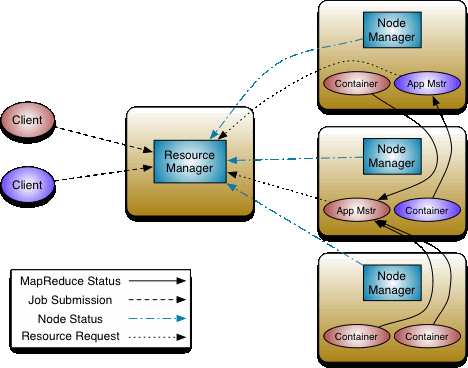
\includegraphics[width=0.5\textwidth]{Figuras/yarn.png}
    \caption{Arquitectura de YARN}
    \label{fig:yarn}
    \source{Imagen extraída de https://hadoop.apache.org/docs/r2.7.2/hadoop-yarn/hadoop-yarn-site/YARN.html}
\end{figure}


\paragraph{HDFS} \textit{Hadoop Distributed File System (HDFS)} es un sistema de archivos que abarca todos los nodos de un \textit{cluster} Hadoop para el almacenamiento de datos. Enlaza entre sí los sistemas de archivos de muchos nodos locales para convertirlos en un único gran sistema de archivos.\cite{quehadoop}

Un \textit{Cluster} HDFS esta compuesto de un \textit{NameNode},un servidor maestro que maneja el espacio de nombres del sistema de archivos y regula el acceso de los clientes a este; y un numero de \textit{DataNodes} que manejan el almacenamiento asociado a los nodos en los que son ejecutados.\cite{horhdfs}

El contenido de los archivos es dividido en grandes bloques (típicamente de 128 megabytes), y cada bloque del archivo es replicado independientemente en múltiples \textit{DataNodes}. Estos son monitoreados activamente por en \textit{NameNode}, que se encarga de replicarlo en caso de perdida.\cite{horhdfs}
El \textit{NameNode} no envía solicitudes directamente a los \textit{DataNodes}. Envia instrucciones a los \textit{DataNodes} replicando a señales enviadas periódicamente por los \textit{DataNodes}.\cite{horhdfs}

Las instrucciones incluyen comandos para: 

\begin{itemize}
    \item Replicar bloques a otros nodos.
    \item Remover copias locales de bloques.
    \item Re-registrar y enviar un reporte de bloques.
    \item Apagar el nodo.
 \end{itemize} The instructions include commands to:



\section{Spark}
Apache Spark es un motor de procesamiento de datos rápido en memoria, permite trabajar de forma eficiente con datos que requieren acceso rápido e iterativo a los conjuntos de datos.\cite{spark}

Consiste en el núcleo Spark y un conjunto de librerías. El núcleo es el métodos de ejecución distribuida, y las APIs de los lenguajes Java, Scala y Python ofrecen una plataforma para el desarrollo de aplicaciones distribuidas. Diferentes librerías adicionales desarrolladas sobre el núcleo aportan diferentes formas de trabajo para el manejo de datos. La habilidad de Spark para mantener los conuntos de datos en memoria principal a manera de cache acelera los procesos iterativos de tratamiento de datos, haciendolo ideal para la implementacion de algoritmos como los utilizados en \textit{Machine Learning}.\cite{spark}


Spark incluye la librería MLlib, la cual provee un conjunto creciente de algoritmos comúnmente usados en técnicas de ciencia de datos tales como : clasificación, regresión, filtros colaborativos, agrupamiento (\textit{clustering}), reducción de dimensionalidad.\cite{spark}

Una de las principales ventajas de Spark es su flexibilidad, puede ejecutarse junto a Hadoop a traves de  YARN y procesar data en HDFS, HBase, Cassandra, Hive, y cualquier otro formato de entrada de Hadoop.\cite{spark}
